\section*{Question 1}
(1) \textit{kernel1Train.csv} contains training data with 1,000 samples, where each sample has two coordinates and the corresponding class. \textit{kernel1Test.csv} contains testing data with 10,000 samples and the same feature space as the training data. The testing data has been reshaped to a $100 \times 100$ grid and a visualization of this grid is shown below in Figure 1.
\begin{figure}[h]
    \centering
    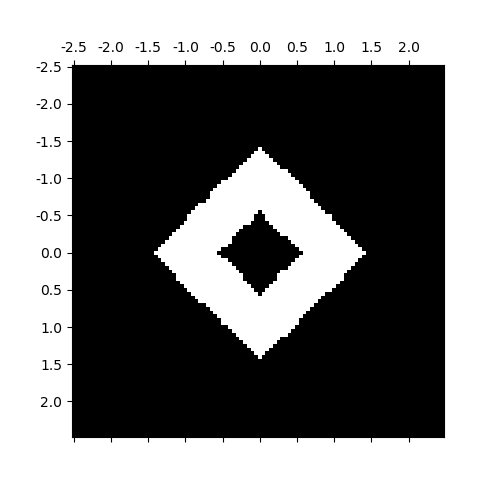
\includegraphics[height=4in]{Figure_1.png}
    \caption{The test set visualized as a $100 \times 100$ grid ranging from -2.5 to 2.45 on both axes. The black cells correspond to a class of 0 and the white cells correspond to a class of 1.}
\end{figure}

(2) Using the SVC class in SciKit-learn, we can train an SVM using a pre-defined kernel or a custom kernel that is specified by the user. For this problem, we use the Cauchy kernel, which is defined as:
\begin{center}
    \large{$K_{\sigma}(x, x') = \frac{1}{1 + \frac{|x - x'|^{2}}{\sigma^{2}}}$}
\end{center}
We use the provided training data to train an SVM for different values of $\sigma$. The classifer's error for each value of $\sigma$ is shown below in Table 1. The error is defined as the fraction of incorrectly-predicted classes over the total number of samples tested. The predicted classes for each case are shown below in Figures 2 - 8, all with the same style of visualization that is shown in Figure 1. A $\sigma$ value of 0.1 yields the best classifier that is able to most accurately predict the classes of the test data.
\begin{table}[h]
\centering
 \begin{tabular}{||c c||} 
 \hline
 $\sigma$ & Error \\ [0.5ex] 
 \hline\hline
0.01 & 0.1243 \\
0.025 & 0.0277 \\
0.05 & 0.0157 \\
0.1 & 0.0144 \\
0.5 & 0.0161 \\
1.0 & 0.0217 \\
2.5 & 0.0511 \\ [0.5ex] 
 \hline
 \end{tabular}
 \caption{Classification error for different values of $\sigma$.}
\label{table:1}
\end{table}
\begin{figure}[h]
    \centering
    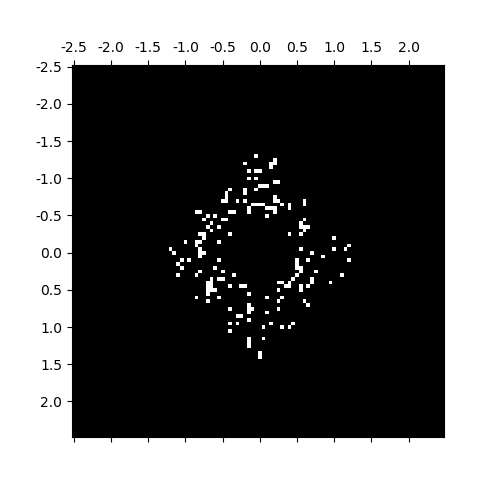
\includegraphics[height=3.5in]{Figure_2_1.png}
    \caption{Predicted classes for $\sigma = 0.01$.}
\end{figure}
\begin{figure}[h]
    \centering
    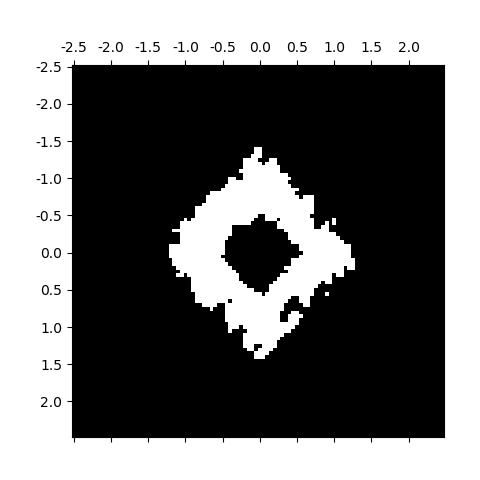
\includegraphics[height=3.5in]{Figure_2_2.png}
    \caption{Predicted classes for $\sigma = 0.025$.}
\end{figure}
\begin{figure}[h]
    \centering
    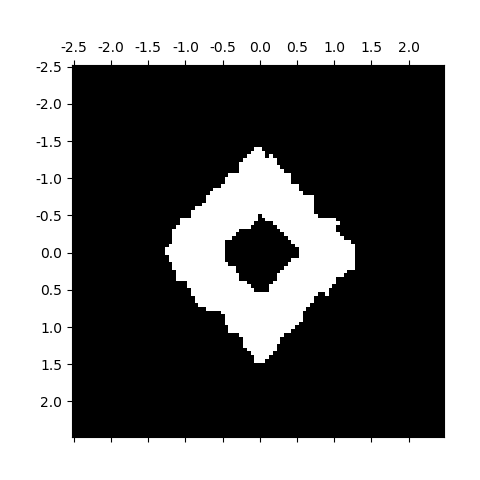
\includegraphics[height=3.5in]{Figure_2_3.png}
    \caption{Predicted classes for $\sigma = 0.05$.}
\end{figure}
\begin{figure}[h]
    \centering
    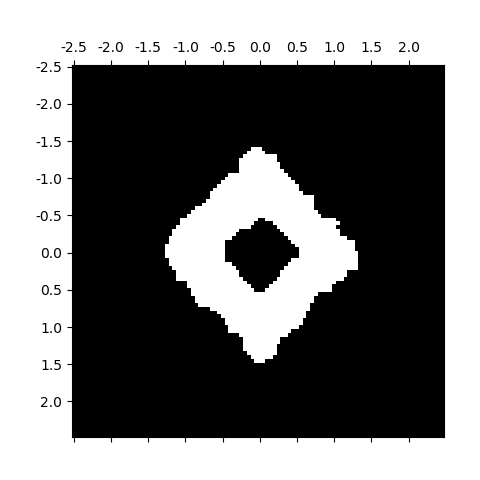
\includegraphics[height=3.5in]{Figure_2_4.png}
    \caption{Predicted classes for $\sigma = 0.1$.}
\end{figure}
\begin{figure}[h]
    \centering
    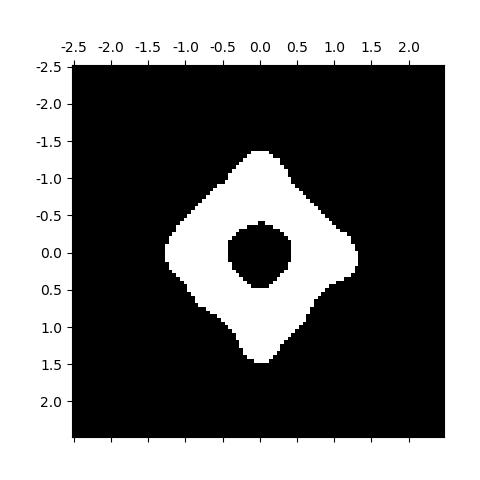
\includegraphics[height=3.5in]{Figure_2_5.png}
    \caption{Predicted classes for $\sigma = 0.5$.}
\end{figure}
\begin{figure}[h]
    \centering
    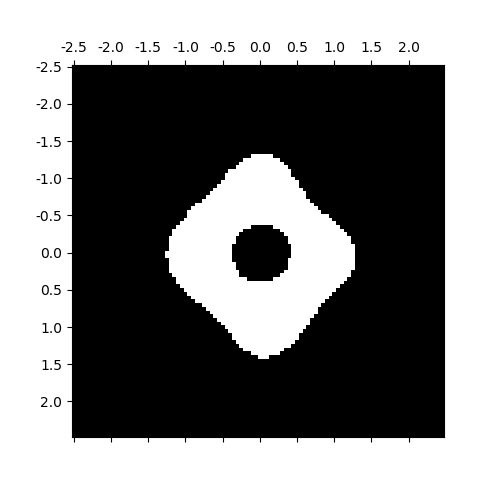
\includegraphics[height=3.5in]{Figure_2_6.png}
    \caption{Predicted classes for $\sigma = 1.0$.}
\end{figure}
\begin{figure}[h]
    \centering
    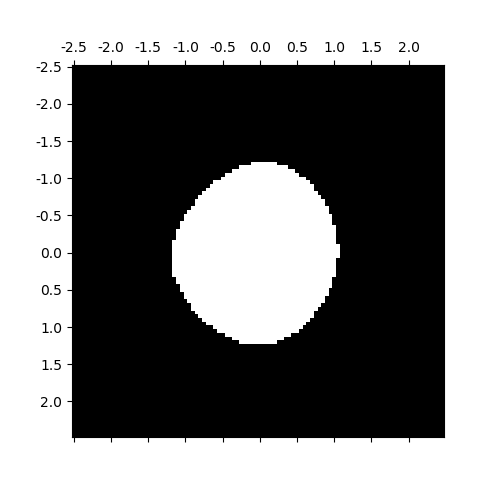
\includegraphics[height=3.5in]{Figure_2_7.png}
    \caption{Predicted classes for $\sigma = 2.5$.}
\end{figure}
\clearpage